\begin{tikzpicture}[
    neuron/.style={circle, fill=black, minimum size=6pt, inner sep=0pt},
    >=stealth
]

% --- Parameters ---
\def\layersep{1.8}
\def\neuronspacing{0.35}
\def\inspacing{0.4}

% Number of neurons per layer
\def\nInput{6}
\def\nHiddenA{11}
\def\nHiddenB{11}
\def\nOutput{6}

% X positions of layers
\def\xInput{0}
\def\xHiddenA{1.8}
\def\xHiddenB{3.6}
\def\xOutput{5.4}


% Input layer
\foreach \i in {1,...,\nInput} {
    \pgfmathsetmacro{\ypos}{(\nInput-1)*\neuronspacing/2 - (\i-1)*\neuronspacing}
    \node[neuron] (I-\i) at (\xInput, \ypos) {};
}

% Hidden layer A
\foreach \i in {1,...,\nHiddenA} {
    \pgfmathsetmacro{\ypos}{(\nHiddenA-1)*\neuronspacing/2 - (\i-1)*\neuronspacing}
    \node[neuron] (HA-\i) at (\xHiddenA, \ypos) {};
}

% Hidden layer B
\foreach \i in {1,...,\nHiddenB} {
    \pgfmathsetmacro{\ypos}{(\nHiddenB-1)*\neuronspacing/2 - (\i-1)*\neuronspacing}
    \node[neuron] (HB-\i) at (\xHiddenB, \ypos) {};
}

% Output layer
\foreach \i in {1,...,\nOutput} {
    \pgfmathsetmacro{\ypos}{(\nOutput-1)*\neuronspacing/2 - (\i-1)*\neuronspacing}
    \node[neuron] (O-\i) at (\xOutput, \ypos) {};
}

% --- Draw connections ---
% Input -> Hidden A
\foreach \i in {1,...,\nInput} {
    \foreach \j in {1,...,\nHiddenA} {
        \draw[gray!50, thin] (I-\i) -- (HA-\j);
    }
}

\draw[thick, dotted] (HA-6.east) -- (HB-6.west);

% Hidden B -> Output
\foreach \i in {1,...,\nHiddenB} {
    \foreach \j in {1,...,\nOutput} {
        \draw[gray!50, thin] (HB-\i) -- (O-\j);
    }
}

% --- Bounding box ---
\draw[thick, rounded corners=3pt]
    ([xshift=-0.4cm, yshift=1.1cm] I-1.north west)
    rectangle
    ([xshift=0.4cm, yshift=-1.1cm] O-\nOutput.south east);

% --- Labels ---

% (a) label
% \node[anchor=north west, font=\bfseries]
    % at ([xshift=-0.25cm, yshift=0.35cm] I-1.north west) {(a)};

% Input label: \tilde{w}(t)
\node[anchor=east, font=\large]
    at ([xshift=-0.7cm] I-3.west) {$\mathbf{z}(t)$};

% Output label: d\tilde{w}(t)/dt
\node[anchor=west, font=\large]
    at ([xshift=0.7cm] O-3.east) {$\dfrac{d\mathbf{z}(t)}{dt}$};

% Network label below
\node[draw, thick, rounded corners=2pt, font=\large,
      anchor=north, inner sep=6pt]
    at ([yshift=-1.5cm] {barycentric cs:I-\nInput=1,O-\nOutput=1})
    {$f_\phi(\mathbf{z}(t))$};

% --- Arrows from box to network label ---
\pgfmathsetmacro{\bottomY}{(\nInput-1.1)*\neuronspacing/2 - (\nInput-1)*\neuronspacing - 1.1}

% Connections from bottom of bounding box to the label box
\coordinate (boxBottom) at (2.7, \bottomY - 0.05);
\coordinate (labelTop) at (2.7, \bottomY - 0.4);

\draw[thick] (boxBottom) -- (labelTop);

\end{tikzpicture}